\flushleft
\begin{minipage}{.75\textwidth}
\begin{Exercise}[label = rotdisk, title = Rotierende Scheibe, difficulty = 2, origin = \url{Jaan Kalda,http://www.ioc.ee/~kalda/ipho/} ]
Die Abbildung zeigt ein Photo einer sich fortbewegenden, rotierenden Scheibe, welches mit langer Belichtungszeit aufgenommen wurde.\\
Die Spur wurde durch eine blaue Lampe beschrieben, welche durchgängliche leuchtet. Gleichzeitig blinkt die Lampe jede  Zehntelsekunde einmal rot auf.\\
Die Lampe ist in einem Abstand von $a =4.5~\mathrm{cm}$ vom Scheibenmittelpunkt montiert.\\
Wie groß ist die Geschwindigkeit des Scheibenmittelpunkts?t
\end{Exercise}
\end{minipage}
\hfill
\begin{minipage}{.2\textwidth}
	\centering
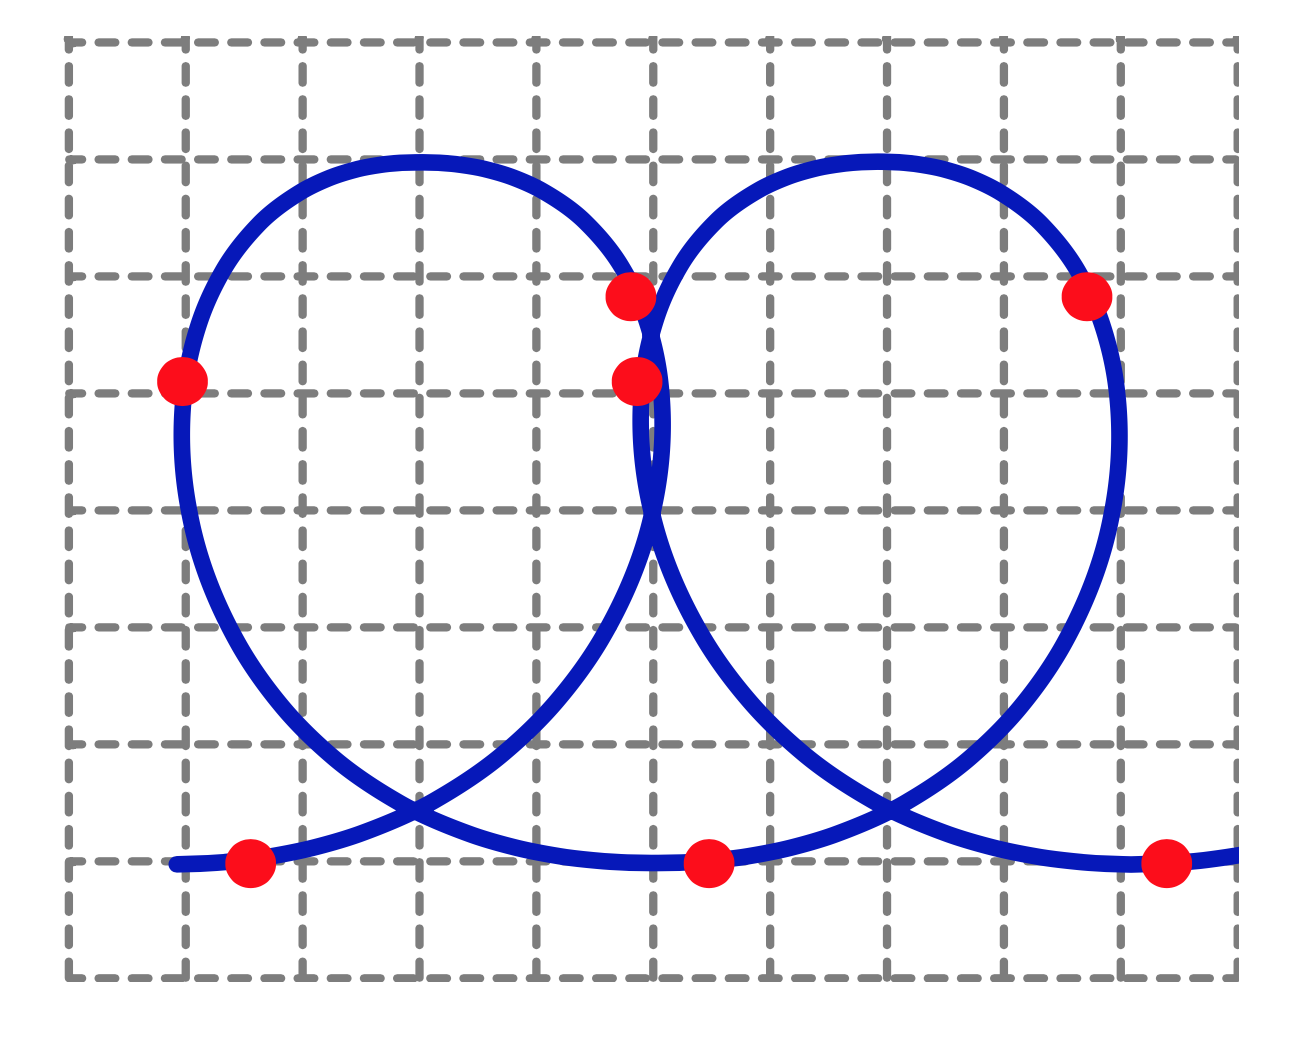
\includegraphics[scale = .2]{../tasks/kalda/rotdisk.png}
\end{minipage}
\begin{Answer}[ref = rotdisk]
	Es fällt auf, dass sich die blaue Bahn nach dem mittleren Punkt unten die Bewegung der Scheibe anscheind widerholt. Da bis dahin die Lampe genau drei Mal geblinkt hat, hat die Scheibe diese Strecke also in einer Zeit von 
	\begin{equation}\label{rotdisk:timeneed}
	T = 3t =0.3~\mathrm{sec}
	\end{equation}
	
	zurückgelegt, wobei $t = 0.1~\mathrm{sec}$ die Zeit ist, die zwischen dem Aufblinken der roten Lampe vergeht.\\
	Diese von der Scheibe zurückgelegte Strecke entspricht in etwa 4 Skaleneinheiten auf dem Bild. Gleichzeitig ist der Abstand zwischen dem untersten Punkt der blauen Bahn, und damit der untersten Position der Lampe, und dem obersten Teil der blauen Bahn, und damit der obersten Position der Lampe, 6 Skaleneinheiten lang. Aber der Abstand zwischen der obersten und der untersten Position der blauen Lampe entspricht genau $2a = 9~\mathrm{cm}$. Also ist eine Skaleneinheit genau $1.5~\mathrm{cm}$ lang. Somit ist die zurückgelegte Strecke $s = 6~\mathrm{cm}$. Für die Geschwindigkeit ergibt sich, mit\eqref{rotdisk:timeneed}
	\begin{equation}
	v = \frac{s}{T} =  \frac{6~\mathrm{cm}}{0.3~\mathrm{sec}} = 20~\mathrm{\frac{cm}{sec}}.
	\end{equation}
\end{Answer}